\RequirePackage[l2tabu,orthodox]{nag}

% TODO: decide if one-sided/two-sided
%\documentclass[headsepline,footsepline,footinclude=false,fontsize=11pt,paper=a4,listof=totoc,bibliography=totoc,BCOR=12mm,DIV=12]{scrbook} % two-sided % original source stated: BCOR=12mm,DIV=12
\documentclass[headsepline,footsepline,footinclude=false,oneside,fontsize=11pt,paper=a4,listof=totoc,bibliography=totoc,DIV=12]{scrbook} % one-sided

% TODO: change citation style in settings
\PassOptionsToPackage{table,svgnames,dvipsnames}{xcolor}

\usepackage[utf8]{inputenc}
\usepackage[T1]{fontenc}
\usepackage[sc]{mathpazo}
\usepackage[ngerman,english]{babel} % english is the same as american or USenglish
\usepackage[autostyle]{csquotes}
\usepackage[%
  backend=biber,
  url=true,
  style=numeric, % alphabetic, numeric
  sorting=none, % default == nty, https://tex.stackexchange.com/questions/51434/biblatex-citation-order
  maxnames=4,
  minnames=3,
  maxbibnames=99,
  giveninits,
  uniquename=init]{biblatex} % TODO: adapt citation style
\usepackage{graphicx}
\usepackage{scrhack} % necessary for listings package
\usepackage{listings}
\usepackage{lstautogobble}
\usepackage{tikz}
\usepackage{pgfplots}
\usepackage{pgfplotstable}
\usepackage{booktabs} % for better looking table creations, but bad with vertical lines by design (package creator despises vertical lines)
\usepackage[final]{microtype}
\usepackage{caption}
\usepackage[hidelinks]{hyperref} % hidelinks removes colored boxes around references and links
\usepackage{ifthen} % for comparison of the current language and changing of the thesis layout
\usepackage{pdftexcmds} % string compare to work with all engines
\usepackage{paralist} % for condensed enumerations or lists
\usepackage{subfig} % for having figures side by side
\usepackage{siunitx} % for physical accurate units and other numerical presentations
\usepackage{multirow} % makes it possible to have bigger cells over multiple rows in a table
\usepackage{array} % different options for table cell orientation
\usepackage{makecell} % allows nice manual configuration of cells with linebreaks in \thead and \makecell with alignments
\usepackage{pdfpages} % for including multiple pages of pdfs
\usepackage{adjustbox} % can center content wider than the \textwidth
\usepackage{tablefootnote} % for footnotes in tables as \tablefootnote
\usepackage{threeparttable} % another way to add footnotes as \tablenotes with \item [x] <your footnote> after setting \tnote{x} 


% https://tex.stackexchange.com/questions/42619/x-mark-to-match-checkmark
\usepackage{amssymb}% http://ctan.org/pkg/amssymb
\usepackage{pifont}% http://ctan.org/pkg/pifont
\newcommand{\cmark}{\ding{51}}%
\newcommand{\xmark}{\ding{55}}%


\usepackage[acronym,xindy,toc]{glossaries} % TODO: include "acronym" if glossary and acronym should be separated
\makeglossaries
\loadglsentries{pages/glossary.tex} % important update for glossaries, before document


\bibliography{bibliography}

\setkomafont{disposition}{\normalfont\bfseries} % use serif font for headings
\linespread{1.05} % adjust line spread for mathpazo font

% Add table of contents to PDF bookmarks
\BeforeTOCHead[toc]{{\cleardoublepage\pdfbookmark[0]{\contentsname}{toc}}}

% Define TUM corporate design colors
% Taken from http://portal.mytum.de/corporatedesign/index_print/vorlagen/index_farben
\definecolor{TUMBlue}{HTML}{0065BD}
\definecolor{TUMSecondaryBlue}{HTML}{005293}
\definecolor{TUMSecondaryBlue2}{HTML}{003359}
\definecolor{TUMBlack}{HTML}{000000}
\definecolor{TUMWhite}{HTML}{FFFFFF}
\definecolor{TUMDarkGray}{HTML}{333333}
\definecolor{TUMGray}{HTML}{808080}
\definecolor{TUMLightGray}{HTML}{CCCCC6}
\definecolor{TUMAccentGray}{HTML}{DAD7CB}
\definecolor{TUMAccentOrange}{HTML}{E37222}
\definecolor{TUMAccentGreen}{HTML}{A2AD00}
\definecolor{TUMAccentLightBlue}{HTML}{98C6EA}
\definecolor{TUMAccentBlue}{HTML}{64A0C8}

% Settings for pgfplots
\pgfplotsset{compat=newest}
\pgfplotsset{
  % For available color names, see http://www.latextemplates.com/svgnames-colors
  cycle list={TUMBlue\\TUMAccentOrange\\TUMAccentGreen\\TUMSecondaryBlue2\\TUMDarkGray\\},
}

% Settings for lstlistings

% Use this for basic highlighting
\lstset{%
  basicstyle=\ttfamily,
  columns=fullflexible,
  autogobble,
  keywordstyle=\bfseries\color{TUMBlue},
  stringstyle=\color{TUMAccentGreen}
}

% use this for C# highlighting
% %\setmonofont{Consolas} %to be used with XeLaTeX or LuaLaTeX
% \definecolor{bluekeywords}{rgb}{0,0,1}
% \definecolor{greencomments}{rgb}{0,0.5,0}
% \definecolor{redstrings}{rgb}{0.64,0.08,0.08}
% \definecolor{xmlcomments}{rgb}{0.5,0.5,0.5}
% \definecolor{types}{rgb}{0.17,0.57,0.68}

% \lstset{language=[Sharp]C,
% captionpos=b,
% %numbers=left, % numbering
% %numberstyle=\tiny, % small row numbers
% frame=lines, % above and underneath of listings is a line
% showspaces=false,
% showtabs=false,
% breaklines=true,
% showstringspaces=false,
% breakatwhitespace=true,
% escapeinside={(*@}{@*)},
% commentstyle=\color{greencomments},
% morekeywords={partial, var, value, get, set},
% keywordstyle=\color{bluekeywords},
% stringstyle=\color{redstrings},
% basicstyle=\ttfamily\small,
% }

% Settings for search order of pictures
\graphicspath{
    {logos/}
    {figures/}
}

% Set up hyphenation rules for the language package when mistakes happen
\babelhyphenation[english]{
an-oth-er
ex-am-ple
}

% Decide between
%\newcommand{\todo}[1]{\textbf{\textsc{\textcolor{TUMAccentOrange}{(TODO: #1)}}}} % for one paragraph, otherwise error!
%\newcommand{\done}[1]{\textit{\textsc{\textcolor{TUMAccentBlue}{(Done: #1)}}}} % for one paragraph, otherwise error!
% and
\newcommand{\todo}[1]{{\bfseries{\scshape{\color{TUMAccentOrange}[(TODO: #1)]}}}} % for multiple paragraphs
\newcommand{\done}[1]{{\itshape{\scshape{\color{TUMAccentBlue}[(Done: #1)]}}}} % for multiple paragraphs
% for error handling of intended behavior in your latex documents.

\newcommand{\tabitem}{~~\llap{\textbullet}~~}

\newcolumntype{P}[1]{>{\centering\arraybackslash}p{#1}} % for horizontal alignment with limited column width
\newcolumntype{M}[1]{>{\centering\arraybackslash}m{#1}} % for horizontal and vertical alignment with limited column width
\newcolumntype{L}[1]{>{\raggedright\arraybackslash}m{#1}} % for vertical alignment left with limited column width
\newcolumntype{R}[1]{>{\raggedleft\arraybackslash}m{#1}} % for vertical alignment right with limited column width

% TODO: change thesis information
\newcommand*{\getUniversity}{Technische Universität München}
\newcommand*{\getFaculty}{Department of Informatics}
\newcommand*{\getTitle}{Anomaly Detection for the Behavior of Drivers B
ased on Structural Temporal Graph Neural Networks}
\newcommand*{\getTitleGer}{Erkennung von Anomalien im Verhalten von Autofahrern auf der Grundlage struktureller temporaler neuronaler Netze}
\newcommand*{\getAuthor}{Hanxi Jiang}
\newcommand*{\getDoctype}{Master's Thesis in Informatics: Robotics, Cognition, Intelligence}
\newcommand*{\getSupervisor}{Supervisor}
\newcommand*{\getAdvisor}{Advisor}
\newcommand*{\getSubmissionDate}{\today}
\newcommand*{\getSubmissionLocation}{Munich}
\addbibresource{bibliography.bib}

\begin{document}

% TODO: decide on used language
%\selectlanguage{ngerman}
\selectlanguage{english}

% Set page numbering to avoid "destination with the same identifier has been already used" warning for cover page.
% (see https://en.wikibooks.org/wiki/LaTeX/Hyperlinks#Problems_with_Links_and_Pages).
\pagenumbering{alph}
\begin{titlepage}
  % HACK for two-sided documents: ignore binding correction for cover page.
  % Adapted from Markus Kohm's KOMA-Script titlepage=firstiscover handling.
  % See http://mirrors.ctan.org/macros/latex/contrib/koma-script/scrkernel-title.dtx,
  % \maketitle macro.
  \oddsidemargin=\evensidemargin\relax
  \textwidth=\dimexpr\paperwidth-2\evensidemargin-2in\relax
  \hsize=\textwidth\relax

  \centering

  \IfFileExists{logos/tum.pdf}{%
    
\includegraphics[height=20mm]{logos/tum.pdf}
  }{%
    \vspace*{20mm}
  }

  \vspace{5mm}
  {\huge\MakeUppercase{\getFaculty{}}}\\

  \vspace{5mm}
  {\large\MakeUppercase{\getUniversity{}}}\\

  \vspace{20mm}
  {\Large \getDoctype{}}

  \vspace{15mm}
  \makeatletter
  \ifthenelse{\pdf@strcmp{\languagename}{english}=0}
  {\huge\bfseries \getTitle{}}
  {\huge\bfseries \getTitleGer{}}
  \makeatother

  \vspace{15mm}
  {\LARGE \getAuthor{}}

  \IfFileExists{logos/faculty.png}{%
    \vfill{}
    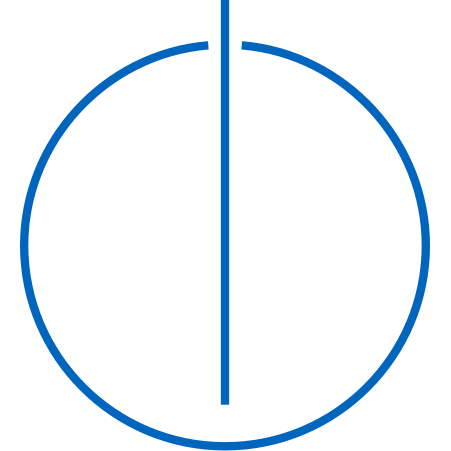
\includegraphics[height=20mm]{logos/faculty.png}
  }{}
\end{titlepage}


\frontmatter{}

\begin{titlepage}
  \centering

  \IfFileExists{logos/tum.pdf}{%
    
\includegraphics[height=20mm]{logos/tum.pdf}
  }{%
    \vspace*{20mm}
  }

  \vspace{5mm}
  {\huge\MakeUppercase{\getFaculty{}}}\\

  \vspace{5mm}
  {\large\MakeUppercase{\getUniversity{}}}\\

  \vspace{20mm}
  {\Large \getDoctype{}}

  \makeatletter
  \vspace{15mm}
  \ifthenelse{\pdf@strcmp{\languagename}{english}=0}
  {
  {\huge\bfseries \getTitle{}}

  \vspace{10mm}
  {\huge\bfseries \foreignlanguage{ngerman}{\getTitleGer{}}}
  }
  {
  {\huge\bfseries \getTitleGer{}}

  \vspace{10mm}
  {\huge\bfseries \foreignlanguage{english}{\getTitle{}}}
  }
  \makeatother

  \vspace{15mm}
  \begin{tabular}{l l}
    Author:          & \getAuthor{} \\
    Supervisor:      & \getSupervisor{} \\
    Advisor:         & \getAdvisor{} \\
    Submission Date: & \getSubmissionDate{} \\
  \end{tabular}

  \IfFileExists{logos/faculty.png}{%
    \vfill{}
    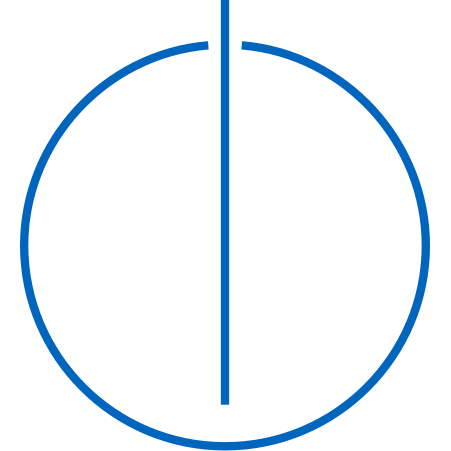
\includegraphics[height=20mm]{logos/faculty.png}
  }{}
\end{titlepage}

\cleardoublepage{}

\thispagestyle{empty}
\vspace*{0.8\textheight}
\noindent
\makeatletter
\ifthenelse{\pdf@strcmp{\languagename}{english}=0}
{I confirm that this \MakeLowercase{\getDoctype{}} is my own work and I have documented all sources and material used.}
{Ich versichere, dass ich diese \getDoctype{} selbstständig verfasst und nur die angegebenen Quellen und Hilfsmittel verwendet habe.}
\makeatother

\vspace{15mm}
\noindent
\getSubmissionLocation{}, \getSubmissionDate{} \hspace{50mm} \getAuthor{}

\cleardoublepage{}

\makeatletter
\ifthenelse{\pdf@strcmp{\languagename}{english}=0}
{\addcontentsline{toc}{chapter}{Acknowledgments}}
{\addcontentsline{toc}{chapter}{Danksagungen}}
\makeatother
\thispagestyle{empty}

\vspace*{20mm}

\begin{center}
\makeatletter
\ifthenelse{\pdf@strcmp{\languagename}{english}=0}
{\usekomafont{section} Acknowledgments}
{\usekomafont{section} Danksagungen}
\makeatother
\end{center}

\vspace{10mm}

%TODO: Acknowledgments

\cleardoublepage{}
 % TODO: if you don't have anyone to thank for or don't wish to publish it, comment this line out.
\chapter{\abstractname}

Despite significant advancements in autonomous driving, improving driving safety remains a critical focus. Researches have demonstrated the potential to detect risks by monitoring elements such as driver behavior and the surrounding environment. However, no specific method has incorporated logistic sequential analysis for future predictions. In this thesis, I propose a novel approach to anomaly detection in driver behavior using dynamic graphs. I selected JODIE, a model well-suited to capturing driver-object interactions due to its compatibility with our dataset structure. To enhance prediction capabilities, I adapted JODIE by incorporating state attributes into graph edges. The modified model predicts not only the edges that would appear but also their associated attributes in the next time sequence. I collected and organized video data of driver participants into dynamic graphs, which represent interactions between drivers and objects over time. These dynamic graphs were then used to train and evaluate the adapted model. Our approach achieved promising performance in detecting anomalies in driver behavior. The results include predictions of object the interactions would contain and the corresponding behavior types. Such outcomes would be more detailed and provide valuable insights into potential risks. This work presents a potential solution for advancing autonomous driving systems, contributing to safer driving environments.



\makeatletter
\ifthenelse{\pdf@strcmp{\languagename}{english}=0}
{\renewcommand{\abstractname}{Kurzfassung}}
{\renewcommand{\abstractname}{Abstract}}
\makeatother

\chapter{\abstractname}

%TODO: Abstract in other language
\begin{otherlanguage}{ngerman} % TODO: select other language, either ngerman or english !
    Trotz erheblicher Fortschritte beim autonomen Fahren bleibt die Verbesserung der Fahrsicherheit ein wichtiger Schwerpunkt. Es wurde gezeigt, dass Methoden zur Erkennung von Risiken durch die Überwachung von Elementen wie dem Fahrerverhalten und der Umgebung möglich sind. Allerdings hat keine spezifische Forschung die logistische sequentielle Analyse für zukünftige Vorhersagen einbezogen. In dieser Arbeit schlagen wir einen neuartigen Ansatz zur Erkennung von Anomalien im Fahrerverhalten unter Verwendung dynamischer Graphen vor, der eine neue Perspektive auf dieses Thema bietet. Nach der Evaluierung modernster dynamischer Graphen-Lernmodelle haben wir uns für JODIE entschieden, ein Modell, das sich aufgrund seiner Kompatibilität mit der Struktur unseres Datensatzes gut für die Erfassung von Fahrer-Objekt-Interaktionen eignet. Um die Vorhersagefähigkeiten zu verbessern, haben wir JODIE angepasst, indem wir Zustandsattribute in die Graphenkanten aufgenommen haben. Das modifizierte Modell sagt nicht nur die Kanten voraus, die in der nächsten Zeitsequenz auftreten werden, sondern auch die zugehörigen Attribute. Hier haben wir Videodaten von Fahrern gesammelt und in dynamische Graphen organisiert, die die Interaktionen zwischen Fahrern und Objekten über die Zeit darstellen. Diese dynamischen Graphen wurden dann zum Trainieren und Bewerten des angepassten Modells verwendet. Unser Ansatz erzielte eine vielversprechende Leistung bei der Erkennung von Anomalien im Fahrerverhalten. Die Ergebnisse umfassen Vorhersagen zu den Objekten, die in den Interaktionen enthalten sind, und zu den entsprechenden Verhaltenstypen. Solche Ergebnisse wären detaillierter und würden wertvolle Erkenntnisse über potenzielle Risiken liefern. Diese Arbeit stellt eine potenzielle Lösung für die Weiterentwicklung autonomer Fahrsysteme dar und trägt zu einer sichereren Fahrumgebung bei.

\end{otherlanguage}


% Undo the name switch
\makeatletter
\ifthenelse{\pdf@strcmp{\languagename}{english}=0}
{\renewcommand{\abstractname}{Abstract}}
{\renewcommand{\abstractname}{Kurzfassung}}
\makeatother
\microtypesetup{protrusion=false}
\tableofcontents{}
\microtypesetup{protrusion=true}

\mainmatter{}

% !TeX root = ../main.tex

\chapter{Introduction}\label{chapter:introduction}
Use with pdfLaTeX and Biber.

\section{contribution}
% Citation test (with Biber)~\parencite{latex}.

\section{Structure}

\subsection{Subsection}

See~\autoref{tab:sample}, \autoref{fig:sample-drawing}, \autoref{fig:sample-plot}, \autoref{fig:sample-listing}, \autoref{fig:tum}, \autoref{fig:tumslide}.

\begin{table}[htpb]
  \caption[Example table]{An example for a simple table.}\label{tab:sample}
  \centering
  \begin{tabular}{l l l l}
    \toprule
      A & B & C & D \\
    \midrule
      1 & 2 & 1 & 2 \\
      2 & 3 & 2 & 3 \\
    \bottomrule
  \end{tabular}
\end{table}

\begin{figure}[htpb]
  \centering
  % This should probably go into a file in figures/
  \begin{tikzpicture}[node distance=3cm]
    \node (R0) {$R_1$};
    \node (R1) [right of=R0] {$R_2$};
    \node (R2) [below of=R1] {$R_4$};
    \node (R3) [below of=R0] {$R_3$};
    \node (R4) [right of=R1] {$R_5$};

    \path[every node]
      (R0) edge (R1)
      (R0) edge (R3)
      (R3) edge (R2)
      (R2) edge (R1)
      (R1) edge (R4);
  \end{tikzpicture}
  \caption[Example drawing]{An example for a simple drawing.}\label{fig:sample-drawing}
\end{figure}

\begin{figure}[htpb]
  \centering

  \pgfplotstableset{col sep=&, row sep=\\}
  % This should probably go into a file in data/
  \pgfplotstableread{
    a & b    \\
    1 & 1000 \\
    2 & 1500 \\
    3 & 1600 \\
  }\exampleA
  \pgfplotstableread{
    a & b    \\
    1 & 1200 \\
    2 & 800 \\
    3 & 1400 \\
  }\exampleB
  % This should probably go into a file in figures/
  \begin{tikzpicture}
    \begin{axis}[
        ymin=0,
        legend style={legend pos=south east},
        grid,
        thick,
        ylabel=Y,
        xlabel=X
      ]
      \addplot table[x=a, y=b]{\exampleA};
      \addlegendentry{Example A};
      \addplot table[x=a, y=b]{\exampleB};
      \addlegendentry{Example B};
    \end{axis}
  \end{tikzpicture}
  \caption[Example plot]{An example for a simple plot.}\label{fig:sample-plot}
\end{figure}

\begin{figure}[htpb]
  \centering
  \begin{tabular}{c}
  \begin{lstlisting}[language=SQL]
    SELECT * FROM tbl WHERE tbl.str = "str"
  \end{lstlisting}
  \end{tabular}
  \caption[Example listing]{An example for a source code listing.}\label{fig:sample-listing}
\end{figure}

\begin{figure}[htpb]
  \centering
  
\includegraphics[width=0.8\textwidth]{tum}
  \caption[Something else can be written here for listing this, otherwise the caption will be written!]{Includegraphics searches for the filename without extension first in logos, then in figures.} \label{fig:tum}
\end{figure}

\begin{figure}[htpb]
  \centering
  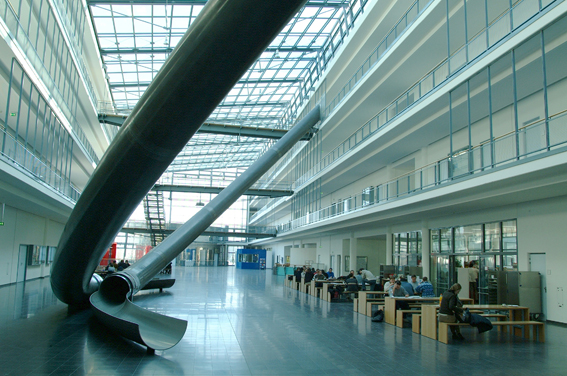
\includegraphics[width=0.8\textwidth]{figures/tum}
  \caption{For pictures with the same name, the direct folder needs to be chosen.} \label{fig:tumslide}
\end{figure}

\begin{figure}[!tbp]
  \centering
  \subfloat[TUM Logo][The logo.]{
\includegraphics[height=0.2\textheight]{tum}\label{fig:tum1}}
  \hfill
  \subfloat[TUM Slide][The famous slide.]{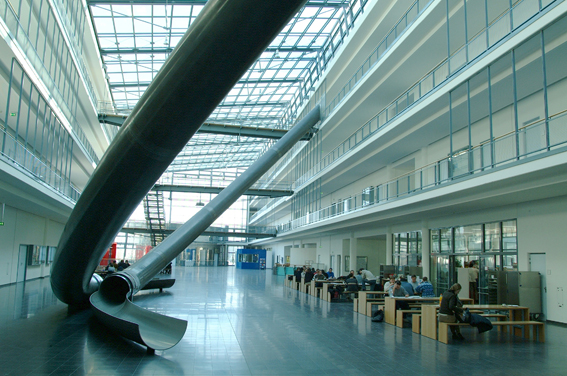
\includegraphics[height=0.2\textheight]{figures/tum}\label{fig:tum2}}
  \caption{Two TUM pictures side by side.}
  \label{fig:sidebyside}
\end{figure}

This is how the glossary will be used.

\Glspl{ddye}, \gls{r0}, \gls{R0}, and \gls{kdeac}. Also, the \glspl{tum} has many \glspl{computer}, not only one \Gls{computer}. Subsequent acronym usage will only print the short version of \glspl{tuma} (take care of plural, if needed!), like here with \gls{tuma}, too. It can also be --> \glsdisp{tum}{hidden}\footnote{Example for a hidden TUM glossary entry.} <--.

\todo{Now it is your turn to write your thesis.

This will be a few tough weeks.}

\done{Nevertheless, celebrate it when it is done!}



\chapter{Background}\label{chapter:background}


\section{Large Language Model}


Large Language Models (LLMs) are highly complex artificial intelligence systems that can learn from the vast amounts of available text data\cite{radford2018improving}. Thanks to the attending of \textit{Transformer}\cite{vaswani2017attention}, a deep learning architecture, these language models which employed self-supervised pre-training have demonstrated improved efficiency and scalability in many fields.

Based on self-attention mechanisms and feed-forward module, \textit{Transformer} has overwhelming advantages in computing representations and global dependencies.

In concrete terms, the Large Language Models equipped with \textit{Transformer} are capable of diverse tasks raised by Natural Language Processing\cite{chowdhary2020natural}, such as textual entailment, question answering, semantic similarity assessment, and document classification. Take BERT\cite{alaparthi2020bidirectional} and GPT\cite{radford2018improving,radford2019language,brown2020language} as two examples, the former utilizes transformer encoder blocks to predict missing words in a given text, and the latter has been enjoying a tremendous reputation for generating diverse and human-like responses, showcasing its potential in various domains.

    \subsection{Text Classification}
In our project, a bunch of hierarchical activity labels would be acquired from the dataset \textit{drive \& act} to depict every detail of the participant's movements in the driving behavior recorded in the video. These labels, however, are too trivial for the construction of learning data, as considering each activity individually will be tedious in such a vast and complex model training process. Therefore, labels should be classified according to the object on which this behavior operates or the specificity of the moment in which the action takes place. For example, the fastening of a seat belt should occur shortly after entering the vehicle, and all behavior related to eating or drinking should be classified into the same group.

In our task, we use zero-shot text classification. This is a task where a model is trained on a set of labeled examples and then classifies new examples from previously unseen classes. This method, which leverages a pre-trained language model, can be thought of as an instance of transfer learning which generally refers to using a model trained for one task in a different application than what it was originally trained for. This is particularly useful for situations where the amount of labeled data is small, for example, our work with 39 different behaviors to be classified.

The model used in the pipeline is \textit{BART} \cite{lewis2019bartdenoisingsequencetosequencepretraining}. According to the paper, BART is trained by corrupting text with an arbitrary noising function and learning a model to reconstruct the original text. It uses a standard Tranformer-based neural machine translation architecture, which, despite its simplicity, can be seen as generalizing BERT (due to the bidirectional encoder), GPT (with the left-to-right decoder), and many other more recent pre-training schemes. With all these prerequisites, it is quite obvious that \textit{BART} is a very practical model for our classification task.

\section{Graph}
\label{sec:graph}
In graph theory, a graph is a structure made up of a collection of objects, where certain pairs of these objects are connected in a specific way\cite{zhou2020graph}. As a powerful tool for modeling and analyzing complex systems, researchers have combined graph theory with deep learning to solve various problems in different fields, such as social networks\cite{wu2020graph}, complex physic system\cite{sanchez2018graph} and Protein-protein interactions (PPIs)\cite{NIPS2017_f5077839}.

A Graph is $\mathcal{G} = (\mathcal{V}, \mathcal{E})$ is a pair of sets, where collections of \textit{nodes} $\mathcal{V}$ and edges $\mathcal{E} \subseteq \mathcal{V}\times \mathcal{V}$ between pairs of nodes. The nodes here are assumed as the nodes to be endowed with s-dimensional \textit{node feature}, denoted by $x_u$ for all $u\in \mathcal{V}$. Taking social network as an example, nodes represent users, and edges correspond to the friendship relations between them. The features of nodes model user properties such as age, likelihood, etc. Also, some models, including this work, would endow the edges with features. In generic setting $\mathcal{E} \neq 0$, the node features are rows of the $x\times d$ matrix $X=(x_1,\ldots,x_n)^T$. To apply some function to update the features in every node, obtaining the set of latent node feature, we would introduce permutation equivariant function $H=F(X)$, where $H$ is the feature matrix whose $u$th row is the latent feature of node $u$.

As for the edges $e\in \mathcal{E}$, or the graph connectivity, they can be represented by the $n\times n$ adjacency matrix $A$ defined as 
\[a_{uv} = \left\{ \begin{array}{rcl}
1 & (u,v)\in \mathcal{E} \\ 0 & otherwise 
\end{array}\right.\]

Here $a_{uv}$  specifies the adjacency information between the nodes described by the $u$th and the $v$th rows of $X$.
Most functions acting on graphs can be viewed as the generators for 'local' node-wise output, i.e., whereby the output on node $u$ directly depends on its neighboring nodes in the graph. It is worthwhile formalizing this constraint explicitly in our model construction by defining what it means for a node to be neighboring another. An (undirected) neighborhood of node $u$ is defined as 
\[\mathcal{N}_u = \{v : (u,v) \in \mathcal{E} \text{ or } (v,u) \in \mathcal{E}\}\]
and the neighborhood features as the multiset\cite{10.48550/arxiv.2104.13478}.
\[\mathcal{X}_{\mathcal{N}_u}={{x_v:v\in N}}\]

Thus, the features of a node as well as its neighborhood could be collected simultaneously by a local function $\phi(x_u,\mathcal{X}_{\mathcal{N}_u}) $. Then the permutation equivariant function $F$ can be constructed by applying $\phi$ to every node's neighborhood in isolation (Figure~\ref{fig:graphupdate}).

$$ F(X,A) = \left[ \begin{array}{rcl}
-- & \phi(x_1,\mathcal{X}_{\mathcal{N}_1}) & -- \\
-- & \phi(x_2,\mathcal{X}_{\mathcal{N}_2}) & -- \\
& \vdots & \\
-- & \phi(x_n,\mathcal{X}_{\mathcal{N}_n}) & --\\

    
\end{array}\right] $$

\begin{figure}[h]
    \centering
    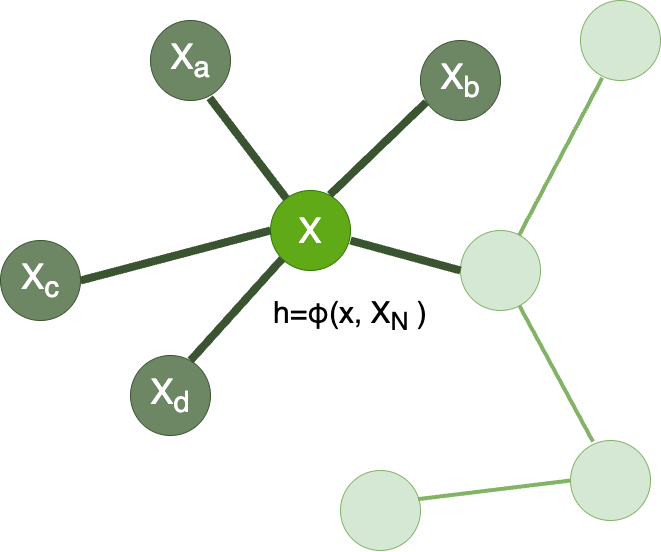
\includegraphics[width=0.5\textwidth]{figures/02_GraphFeature.png}
    \caption{Constructing permutation equivariant functions over graphs.}
    \label{fig:graphupdate}
\end{figure}



    \subsection{Graph Neural Networks}
    The intuitive understanding among \textbf{Graph Neural Network (GNN)} is that nodes in a graph represent objects or concepts, and edges represent their relationships. Each concept is naturally defined by its features and the related concepts\cite{10.1109/tnn.2008.2005605}. GNNs are among the most general class of deep learning architectures currently in existence, and most learning architectures can be understood as a special case of the GNN with additional geometric structure. 
    
    Given to the mathematic expression we have settled in section~\ref{sec:graph} we consider a graph to be specified with an adjacency matrix $A$ and node feature $X$. The GNN architectures we study arepermutation equivariant functions $F(X,A)$  construcetd by applying shared permutation invariant function $\phi(x_u,\mathcal{X}_{\mathcal{N}_u}) $ over local neighborhood. This function $\psi$ would be referred to as "diffusion", "propagation", or "message passing", and the all over computation of such of such $F$ as a "GNN layer".

    The design and study of GNN layers is one of the most active area of deep learning in the recent past few years. And three vast "flavours" of GNN layers are derived from the vast majority of the literatures. These flavours govern the extent to which $\psi$ transforms the neighbourhood features, allowing for varying degrees of complexity when modelling interactions across the graph(Figure~\ref{fig:graphlayer}). 
    
    \begin{figure}[h]
        \centering
        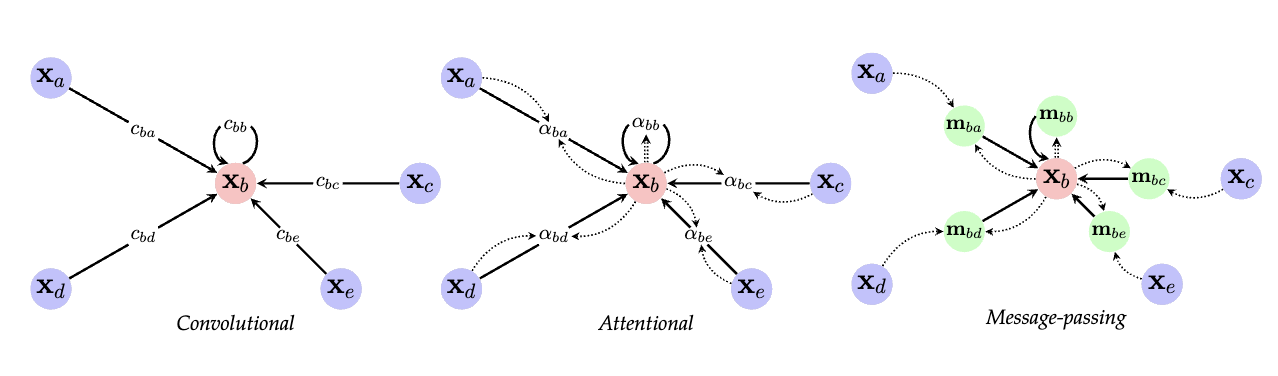
\includegraphics[width=\textwidth]{figures/02_GNNlayers.png}
        \caption{A visualisation of the dataflow for the three flavours of GNNlayers. Reproduced from \cite{10.48550/arxiv.2104.13478}}
        \label{fig:graphlayer}
    \end{figure}

    In all the three flavours, the feature update function for node $u$ would apply permutation-invariant function $\oplus$ to aggregate features from $\mathcal{X}_{\mathcal{N}_u}$ ,as well as learnable function $\psi$. The function $\oplus$ is potentially transformed, by means of some function $\psi$ and itself is usually realized as a nonparametric operation such as sum, mean, or maximum.


    In the \textbf{convolution flavour}\cite{kipf2016semi,defferrard2016convolutional,wu2019simplifying}The feature of the neighborhood nodes are directly aggregated with fixed weights $c_{uv}$, which often directly depends on the entries in $A$ representingthe structure of the graph. The update function is defined as:
    \[
    \mathbf{h}_u = \phi \left( \mathbf{x}_u, \bigoplus_{v \in \mathcal{N}_u} c_{uv} \psi(\mathbf{x}_v) \right).
    \]


    In the \textbf{attention flavour}\cite{velickovic2017graph,monti2017geometric,zhang2018gaan}the weights $c_{uv}$ are replaced by the a learnable self-attention mechanism that computes the importancecoefficients. And the update function is defined as:

    \[
        \mathbf{h}_u = \phi \left( \mathbf{x}_u, \bigoplus_{v \in \mathcal{N}_u} a(x_u,x_v) \psi(\mathbf{x}_v) \right).
    \]

    And the \textbf{message-passing flavour}\cite{gilmer2017neural,battaglia2018relational} aims at computing arbitrary vectors of neighborhood $\mathcal{N}_u$ send to $u$, where vector-based messages are computed based on both the sender and receiver: $m_{uv} = \psi (x_u, x_v)$.
    \[
        \mathbf{h}_u = \phi \left( \mathbf{x}_u, \bigoplus_{v \in \mathcal{N}_u} \psi (x_u, x_v) \right).
    \]

    What matters is that a representational containment between these approaches exists: $convolution \in attention \in message-passing $. This, however, does not mean that message-passing is always the most useful choice. Indeed, the vector-based messages always contains most oriented information across the edges, but they are harder to train due to the enormous requirement of memories. And here, in our work, we have such a specific network that none of the approaches above is the best choice.
 

    \subsection{Dynamic graph}
    Our discussion so far has focused solely on input that exhibits spatial variations across a given domain; however, the input may also change over time, for instance, video, text or speech.
    Assume that the input consists of arbitrary steps, and an input signal will be provided at each step $t$, we represent as $X^{(t) \in \mathcal{X} (\omega^{(t)})}$

    While in many cases the domain in kept fixed across time $t$, we notice that exceptions also happens. For example in our work, we many find tremendous changes in the videos from our dataset. Such domain as changing over time is referred to as \textit{dynamic graph}\cite{rossi2006temporal,xu2020inductive}.

    Assume an encoder function $f(X^(t))$ offering latent presentation for such dynamic graph learning problem. In the video analysis, $\omega$ is a fixed grid, and signals are a sequence of frames. To have a view of the entire frame, one of the options is to implement $f$ as a translation invariant CNN, outputting a k-dimensional representation $z(t)=f(X^(t))$  of the frame at time-step $t$. In our work, however, we use an alternative approaches, which we would introduce in chapter\ref{chapter:relatedwork}.

    To have a canonical analysis for dynamically aggregate the sequence of vectors $z(t)$, we introduce \textit{Recurrent Neural Network} (RNN)\cite{schmidt2019recurrent} due its advantages in the field of temporal progression of inputs and online arrival of novel data-points. A clear view of analyzing video data with RNN is given in Figure~\ref{fig:RNN}.

    \begin{figure}[h]
        \centering
        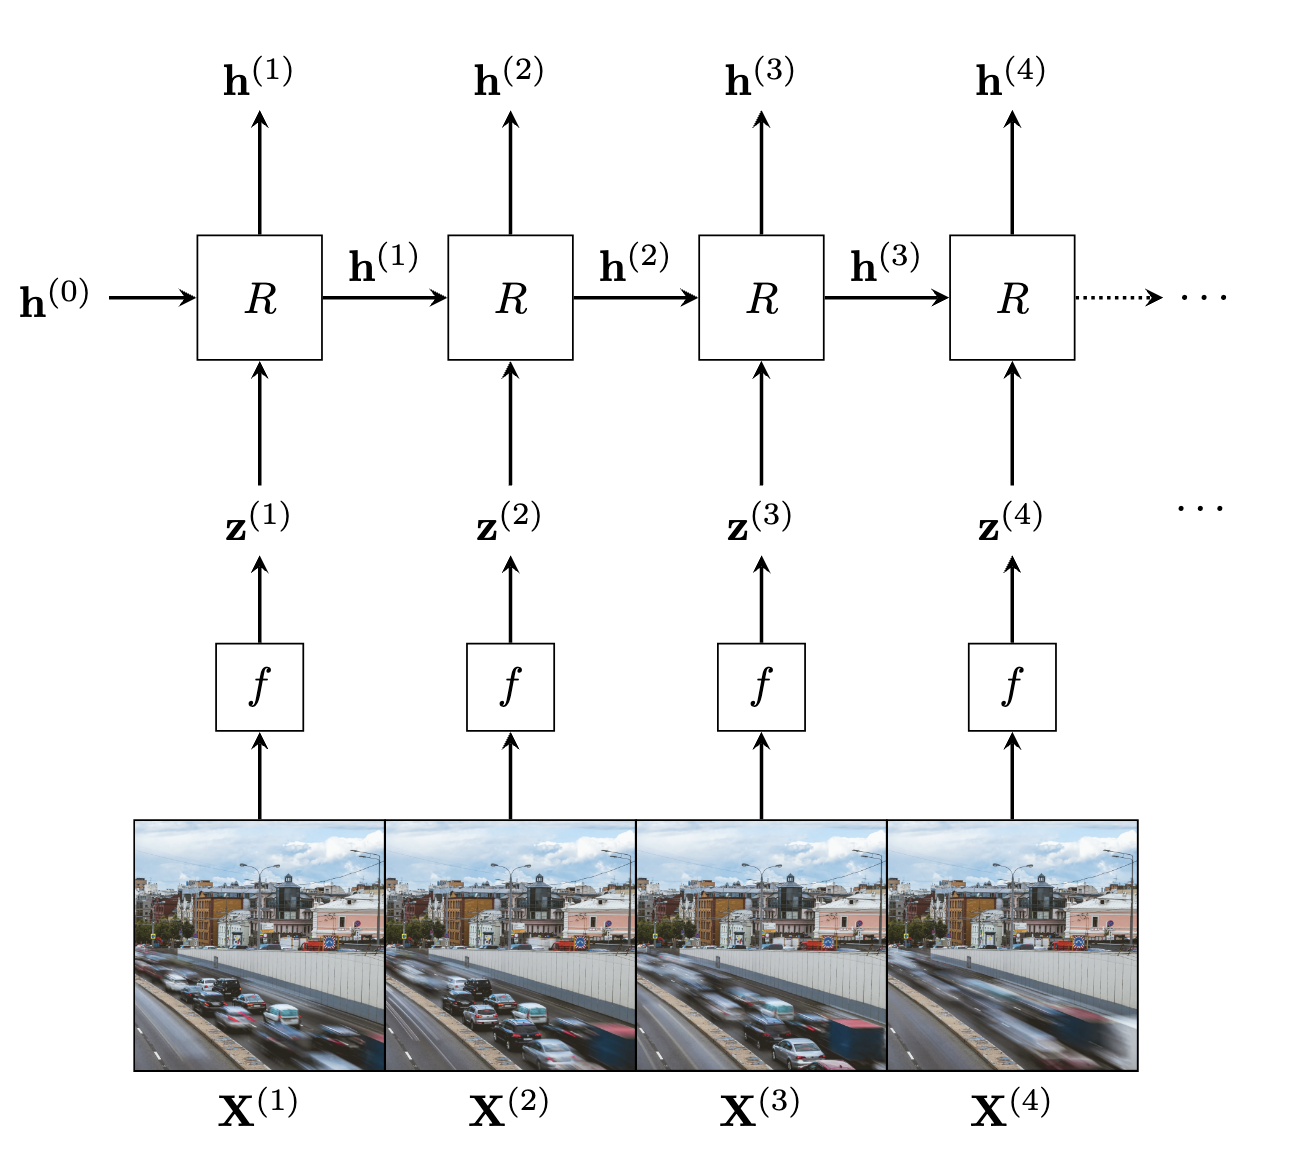
\includegraphics[width=0.7\textwidth]{figures/02_RNN.png}
        \caption{Illustration of processing video input with RNNs. Reproduced from \cite{10.48550/arxiv.2104.13478}}
        \label{fig:RNN}
    \end{figure}

    A simple RNN model is defined as the following way: The model holds with an m-dimensional summary vector $h(t)$ of all the input steps up to and including $t$. This will summarize the current step's features as well as the information collected from the past, through a shared function $R: \mathbb{R} ^k \times \mathbb{R} ^m \rightarrow \mathbb{R} ^m$, as follows:
    \[
        h(t) = R(z(t), h(t-1))
    \]

    As both $z(t)$ and $h(t-1)$ are vectors, the function $R$ is usually realized as a simple feed-forward neural network(often known as \textit{Simple RNN}\cite{elman1990finding,jordan1997serial}):
    \[
        h(t) = \sigma(W_z z(t) + U h(t-1) + b)
    \]
    Where $W_z$ and $U$ are the weight matrices, $b$ is the bias, and $\sigma$ is the activation function. 

    The summary vectors may then be appropriately leveraged for the down-stream task—if a prediction is required at every step of the sequence, then a shared predictor may be applied to each $h(t)$ individually. For classifying entire sequences, typically the final summary, $h(T)$, is passed to a classifier, just like many works including ours.



    

\section{behavior prediction for human driver}

The earliest research regarding the prediction of human driver behavior could be dated back to the 1990s, when hidden Markov models are first introduced to model the driver's behavior\cite{10.1162/089976699300016890}. An HMM is a statistical model that represents a system with hidden states, where observable outputs are generated by these underlying, unobservable states. Each state transitions to another with a certain probability and emits observations based on specific probability distributions. 

The paper is constructed on the ground truth that the intended actions, like to turn or change lanes, are modeled as a sequence of internal states. By observing the temporal patterns of the driver's behavior or even intention. Although the attempt then is to capture and predict driver eye movements in the context of lane keeping/curve negotiation and car following to determine. It still proves that characteristic patterns in driver behavior could be identified and even represent by mathematical models.

With the advancement of various machine learning models, more sophisticated tools have emerged, expanding the range of options available for predicting human driver behavior. In \cite{10.1109/ivs.2018.8500717}, hidden Markov models are adapted for this topic as well, yielding promising results due to the enhanced computational capabilities available today. Another study \cite{10.1109/icra40945.2020.9196918} proposes an LSTM-based trajectory prediction method for human drivers, which facilitates better decision-making for autonomous vehicles, particularly in urban intersection scenarios. Despite these significant achievements, there remains a noticeable gap in driver behavior prediction for driver-oriented dynamic scene graphs. Such an approach could capture individual driving habits, enabling more precise predictions and even anomaly detection tailored to each driver. Our work aims to address this gap.
\chapter{Related Work}\label{chapter:relatedwork}

\section{Datasets for driver behavior analysis}

As of the time of writing, numerous datasets are available for driver behavior analysis, each with its own specific focus. For instance, \textit{DR(eye)VE Dataset}\cite{palazzi2018predicting}capturing drivers' gaze patterns in real-world scenarios, includes ego-centric views and car-centric views, which provide data on where drivers look in different driving contexts. \textit{Naturalistic Driving Study (NDS)}\cite{regan2012naturalistic} contains extensive data collected from naturalistic driving conditions, including in-vehicle driver behavior such as driver movements, eye gaze, and interactions with vehicle controls during different driving scenarios. Detailed information can be found in \ref{chapter:appendix}


In our work, we utilize the \textbf{Drive \& Act} dataset\cite{9009583} as our primary training resource. This dataset includes over twelve hours and 9.6 million frames, capturing individuals engaged in various distractive activities during both manual and automated driving. It is specialized for distinguishing between closely related actions (e.g., opening a bottle vs. closing a bottle) and features a high diversity in action durations and complexities, presenting unique challenges for action recognition models. For instance, brief actions like opening a door from the inside may take less than a second, while prolonged activities such as reading a magazine may last several minutes. This dataset is exceptionally well-suited to our study, as it provides a comprehensive view of driver behavior within the vehicle, with accurately labeled, temporally sequenced annotations for each behavior.


\begin{figure}
    \centering
    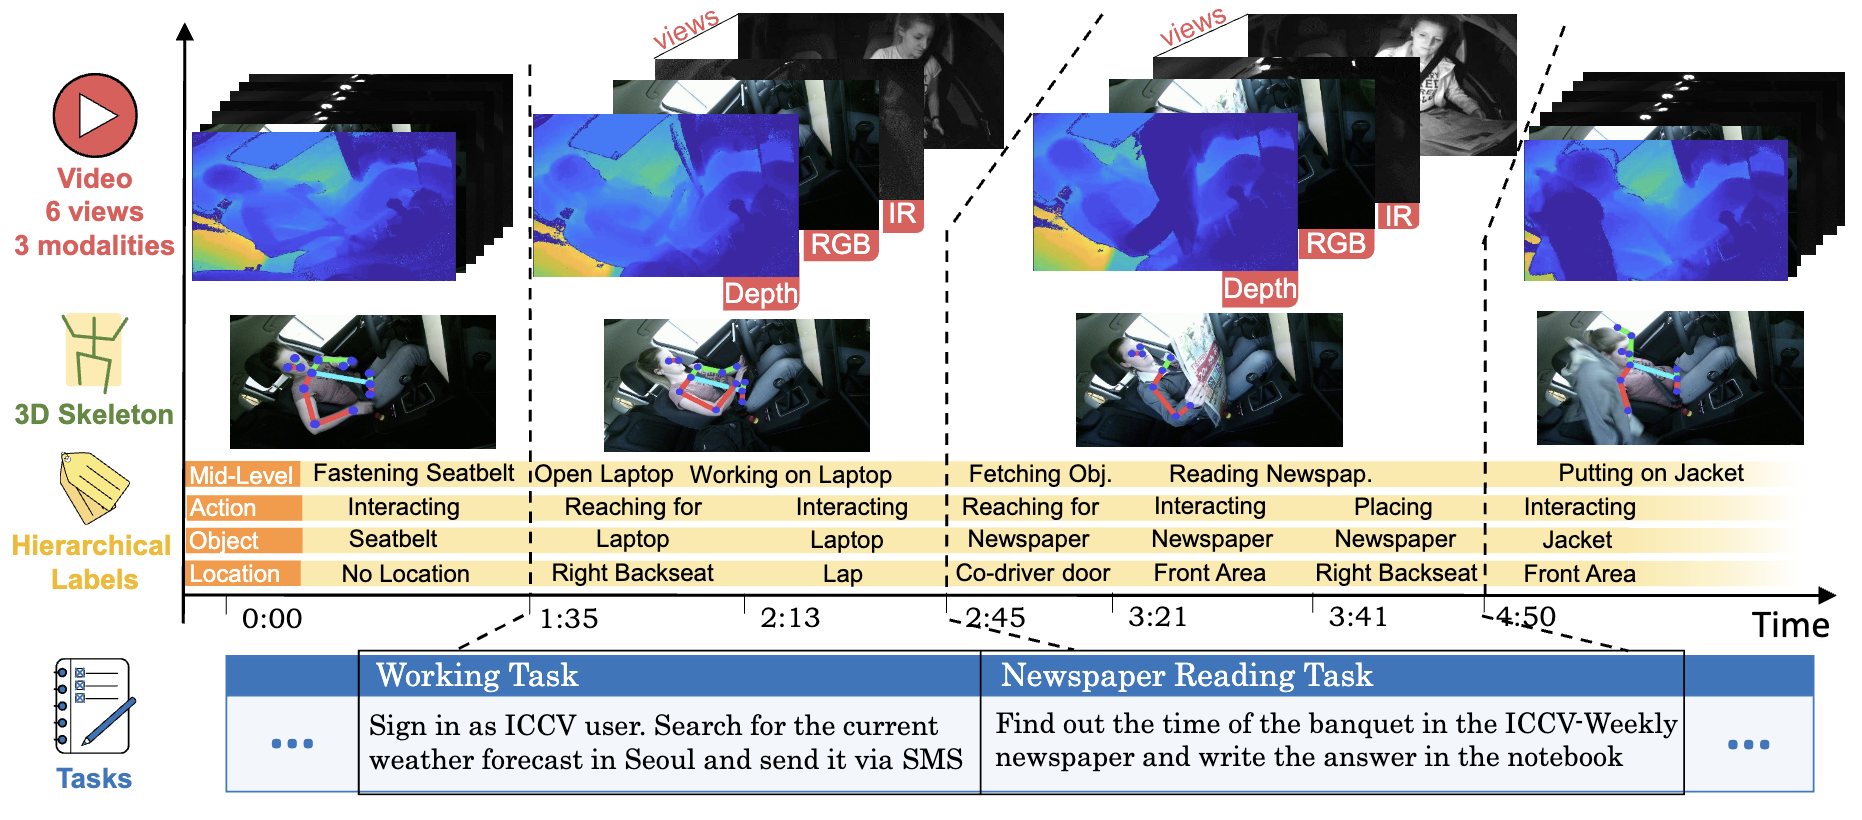
\includegraphics[width=0.8\linewidth]{figures/03_DriveAct.png}
    \caption{Overview of the Drive\&Act dataset for driver behavior recognition. Reproduced from\cite{9009583}}
    \label{fig:DriveAct}
\end{figure}

\section{Dynamic Scene Graph for Video}

As is revealed in chapter~\ref{chapter:background}, the most common way to represent the latent information in a video is to use CNNs to directly extract the features of the frames and then use RNNs to model the temporal information. However, this method has its limitations as the excessive high-dimensional abstraction may cause the model to misinterpret human learning intentions; in other words, the black box itself is difficult to interpret. In our work we would like to extract the dynamic scene graph from the video, which is a more intuitive way to represent the video content.

The scene graph is a structured representation of a scene that can clearly express the objects, attributes, and relationships between objects in the scene\cite{9661322}. Accompanied by the development of computer vision technology, simply detecting and recognizing objects in images no longer satisfies the researchers, as they would expect some higher level of understanding and reasoning for image vision tasks. In this way, an intuitive idea comes up about adding up the relationship between the detected objects (See example in figure\ref{fig:SGG}). The earliest research could date back to 2017, when some objects and relations of a given image could be inferred, and a scene graph would be produced as a result\cite{xu2017scene}. Other research like Neural Motifs\cite{zellers2018neural} also shows the possibility of predicting the most frequent relation between object pairs with the given labels and object detections. Later in 2018, videos came into discussion, and both spatial and temporal relations would be concerned in the dynamic graph researchers propose to represent\cite{wang2018videos}. Meanwhile, the accuracy of Scene Graph Detection tasks has significantly improved thanks to the application of unbiased SGG\cite{wang2018videos}, fueled by the \textit{Detection2} \cite{wu2019detectron2}, a library that contains various state-of-the-art detection and segmentation algorithms. In a nutshell, representing videos as dynamic scene graphs including the detection of objects and the relations in between has been realized in the past years. And our work would utilize such technique and extract our driver-oriented dynamic scene graphs for further learning.

\begin{figure}
    \centering
    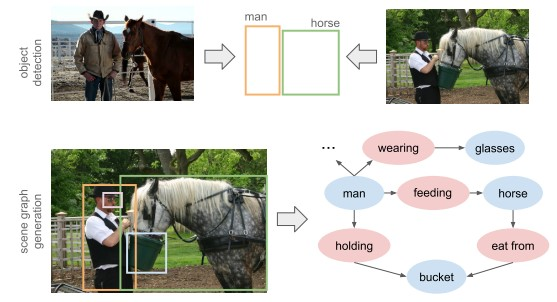
\includegraphics[width=\linewidth]{figures/03_SGG.jpg}
    \caption{Scene Graph Generation by Iterative Message Passing. Reproduced from\cite{tang2020unbiased}}
    \label{fig:SGG}
\end{figure}

\section{Dynamic Link Prediction}


After extracting the dynamic scene graph from video data, the subsequent phase involves learning the interactions between elements within the scene to enable accurate behavior prediction. This objective can be conceptualized as a link prediction task within a dynamic scene graph, making the selection of an appropriate model critical to the success of our approach. Leveraging the review provided in \textit{DGB} \cite{poursafaei2022towards}, we have identified and evaluated various link prediction models along with effective evaluation strategies. Below, we introduce each model and provide a theoretical explanation for our choice.

\subsubsection{ JOINT DYNAMIC USER-ITEMEMBEDDING MODEL(JODIE)}
Based on the user-item interaction data, \textbf{JODIE}\cite{kumar2019predicting} works as a coupled \textit{Recurrent Neural Networks(RNN)}. The update operator alternatively updates the embedding space of suer and an item at each interaction. And the projection operator learns to estimate the embedding of the user at any time in the future, thereby enabling the prediction of forthcoming interactions. The design and functionality of JODIE align well with our objectives, making it a strong candidate for our work.

\subsubsection{Representation Learning over Dynamic Graphs(DyRep)}
\textbf{DyRep}\cite{trivedi2018representation} is an inductive deep representation learning framework that learns a set of functions to efficiently produce low-dimensional node embeddings that evolves over time. The model captures all the new edges appears during the time sequence and updates the embeddings of the nodes accordingly in a custom RNN model. The final output provides a solution to the problems of dynamic link prediction and event time prediction. TGN achieves superior performance over prior models and offers computational efficiency, making it a potential fit for our data, although some constraints exist.


\subsubsection{Temporal Graph Network(TGN)}
\textbf{TGN}\cite{rossi2006temporal} is a generic, efficient framework for deep learning on dynamic graphs represented as sequences of timed events. To train the Memory-related modules, the message matrix would begin with a raw message store and is updated based on interactions which have been processed by the model in the past, which would also propagate to the node embedding as well as the loss function. TGNs significantly outperform previous approaches while being more computationally efficient, Which shows the possibility of applying on our data.

\subsubsection{Causal Anonymous Walks Network (CAW-N)}
Based on \textit{temporal random walks}, \textbf{CAW-N} adopt a novel anonymization strategy that replaces node identities with the hitting counts of the nodes based on a set of sampled walks to keep the method inductive, and simultaneously establish the correlation between motifs. It is specialized in work as automatic retrieval of temporal network motifs to represent network dynamics. Since our dataset has only little similarity with random walking, we didn't take this into consideration at last.


After evaluating each of these models, we selected \textbf{JODIE} as the final model for our work. Theoretically, this choice is justified by the structural similarity of our dataset, which features participant-object interactions akin to user-item data. Although \textbf{TGN } also offers a sophisticated architecture, its need for extensive training data rendered it impractical for our dataset's constraints.
\chapter{Methodology}\label{chapter:methodology}
% NOTE: add HMM as baseline

This work aims to construct a graph neural network-based architecture for predicting, analyzing, and detecting any potentially abnormal behavior regarding the driver during the whole driving process. In particular, The model extracts a description graph, the so-called scene graph, of the driver from the video filmed inside the vehicle and trains itself with these data to learn for future behavior prediction. The result will be used to compare and detect any abnormal behavior. Here we would lay most emphasis on the construction of the training model. To make precious anomaly detection we aim to predict not only if there is a behavior between humans and a specific kind of object but the type of behavior as well, which will cause several adaptions based on existing model \textit{JODIE}.

This chapter will follow the pipeline of the whole work


% advantage




\section{Scene graph generation}

% here we generate the graph directly from table from the row data

    \subsection{Video data extracting}

    \subsection{Graph generating}
% we classify and label the behavior with LLM

\section{Model architecture}
% what is JODIE
As is mentioned in chapter \ref{chapter:relatedwork}, the model \textit{JODIE} is a 

% how do we change the loss function
% we training with the model adapted from JODIE




After comparing all the training results of the below models we would find that **JODIE** is one coming up with the best prediction. However, the model jodie still fail to predict the state of the predicted edge.
In my masterwork I would like to rewrite the embedding function and the loss function of **JODIE to make the state prediction possible.

- function from **JODIE**:

embedding function
$$ \mathbf{u(t)}=\sigma(W_1^u\mathbf{u(t^-)}+W_2^u\mathbf{i(t^-)}+W_3^uf+W^u_4 \Delta _u)$$
$$ \mathbf{i(t)}=\sigma(W_1^i\mathbf{i(t^-)}+W_2^i\mathbf{u(t^-)}+W_3^if+W^i_4 \Delta _i)$$

loss function(BCE)
$$L=-(j_{pos}\log{\tilde{j}}+j_{neg}log(1-\tilde{j}))$$

where

$$\tilde{j}(t+\Delta)=W_1\hat{u}(t+\delta)+W_2\bar{u}+W_3i(t+\Delta ^-)+W_4\bar{i}+B$$



- functions adapted in my work:

embedding function
$$ \mathbf{u(t)}=\sigma(W_1^u\mathbf{u(t^-)}+W_2^u\mathbf{i(t^-)}+W_3^uf+W^u_4s+W^u_5\Delta _u)$$
$$ \mathbf{i(t)}=\sigma(W_1^i\mathbf{i(t^-)}+W_2^i\mathbf{u(t^-)}+W_3^if+W^i_4s+W^u_5 \Delta _i)$$

we will change it from BCE to CE for predictiing state.

$$\tilde{j}(t+\Delta)=W_1\hat{u}(t+\delta)+W_2\bar{u}+W_3i(t+\Delta ^-)+W_4\bar{i}+W_5s+B$$
\chapter{Evaluation}\label{chapter:evaluation}

In the previous chapter(Chapter~\ref{chapter:methodology}), we detailed the entire workflow and underlying mechanisms of our proposed model. This chapter focuses on the evaluation of the results obtained throughout the study, providing an analysis of the model's performance and reasoning about the outcomes achieved.

Given that abnormal behavior detection is just one potential application of the developed model, the evaluation emphasizes its overall performance. Specifically, this chapter will compare results across different models applied to the same video, analyze the performance of the JODIE model on individual videos, evaluate the baseline results using Hidden Markov Models (HMM), and assess the impact of incorporating state embeddings into the JODIE framework.

Table~\ref{tab:dataset_statistic} and figure \ref{fig:dataset_statistic} offers an overview of the dataset used in the study. The dataset originates from experimental videos recorded with 15 participants, each contributing approximately two videos. The duration of each video ranges from 20 to 40 minutes, with each video containing around 13 to 16 nodes and 5000 to 15000 edges.

To further assess the model's scalability and generalization capabilities, we created a combined video by concatenating all the source videos. This combined dataset aims to test whether the model can predict driver behavior across all participants within a single learning process. The combined video has a total duration of approximately 10 hours, with 16 nodes and 287,644 edges. The number of nodes in the dataset shows only slight variation across videos. However, significant differences are observed in the number of edges and the video duration. As such, these latter factors—edge count and video duration—are considered the primary contributors to variations in model performance when applying the same model to different datasets.

Since our goal is to make predictions within dynamic graphs, it is essential to account for both \textbf{old nodes} that have appeared in previous time steps and \textbf{new nodes} that have not yet been observed. Both cases are integral to evaluating the model’s ability to generalize and adapt to evolving graph structures.

\clearpage


\begin{longtable}{lcccc}
        \toprule
    Participators        & Video    & \multicolumn{1}{l}{duration} & Number of Nodes& Number of Edges\\
        \midrule
    all                 & combined & 10:15:31                     & 16    &287644  \\
        \midrule
    \multirow{2}{*}{1}  & vp1\_1   & 00:21:10                     & 14    &8871     \\
                        & vp1\_2   & 00:23:49                     & 14    &8022          \\
        \midrule
    \multirow{2}{*}{2}  & vp2\_1   & 00:25:13                     & 15    &7291          \\
                        & vp2\_2   & 00:22:42                     & 14    &11865          \\
        \midrule
    \multirow{2}{*}{3}  & vp3\_1   & 00:22:22                     & 14    &9086          \\
                        & vp3\_2   & 00:18:11                     & 14    &6298          \\
        \midrule
    \multirow{2}{*}{4}  & vp4\_1   & 00:36:59                     & 15    &15497          \\
                        & vp4\_2   & 00:30:18                     & 15    &8626          \\
        \midrule
    \multirow{2}{*}{5}  & vp5\_1   & 00:29:37                     & 15    &13511          \\
                        & vp5\_2   & 00:21:39                     & 15    &7172          \\
        \midrule
    \multirow{2}{*}{6}  & vp6\_1   & 00:30:01                     & 16    &10056          \\
                        & vp6\_2   & 00:23:47                     & 15    &7878          \\
        \midrule
    \multirow{2}{*}{7}  & vp7\_1   & 00:23:07                     & 15    &9450          \\
                        & vp7\_2   & 00:15:28                     & 13    &5418          \\
        \midrule
    \multirow{2}{*}{8}  & vp8\_1   & 00:25:37                     & 15    &12513          \\
                        & vp8\_2   & 00:22:11                     & 14    &9748          \\
        \midrule
    9                   & vp9\_1   & 00:16:58                     & 14    &9057          \\
        \midrule
    \multirow{2}{*}{10} & vp10\_1  & 00:23:31                     & 15    &10524          \\
                        & vp10\_2  & 00:23:05                     & 13    &7534          \\
        \midrule
    \multirow{2}{*}{11} & vp11\_1  & 00:20:53                     & 11    &9157          \\
                        & vp11\_2  & 00:15:16                     & 13    &7193          \\
        \midrule
    \multirow{2}{*}{12} & vp12\_1  & 00:22:09                     & 16    &10451          \\
                        & vp12\_2  & 00:28:11                     & 15    &14807          \\
        \midrule
    \multirow{2}{*}{13} & vp13\_1  & 00:25:51                     & 13    &9518          \\
                        & vp13\_2  & 00:22:37                     & 14    &8319          \\
        \midrule
    \multirow{2}{*}{14} & vp14\_1  & 00:27:19                     & 14    &15539          \\
                        & vp14\_2  & 00:24:49                     & 13    &13889          \\
        \midrule
    \multirow{2}{*}{15} & vp15\_1  & 00:25:46                     & 14    &6873          \\
                        & vp15\_2  & 00:21:55                     & 13    &7621          \\
        \bottomrule

    \caption{The statistic of the dynamic graph derived from the source videos}
    \label{tab:dataset_statistic}
\end{longtable}

\clearpage
\begin{figure}[h]
    \centering
    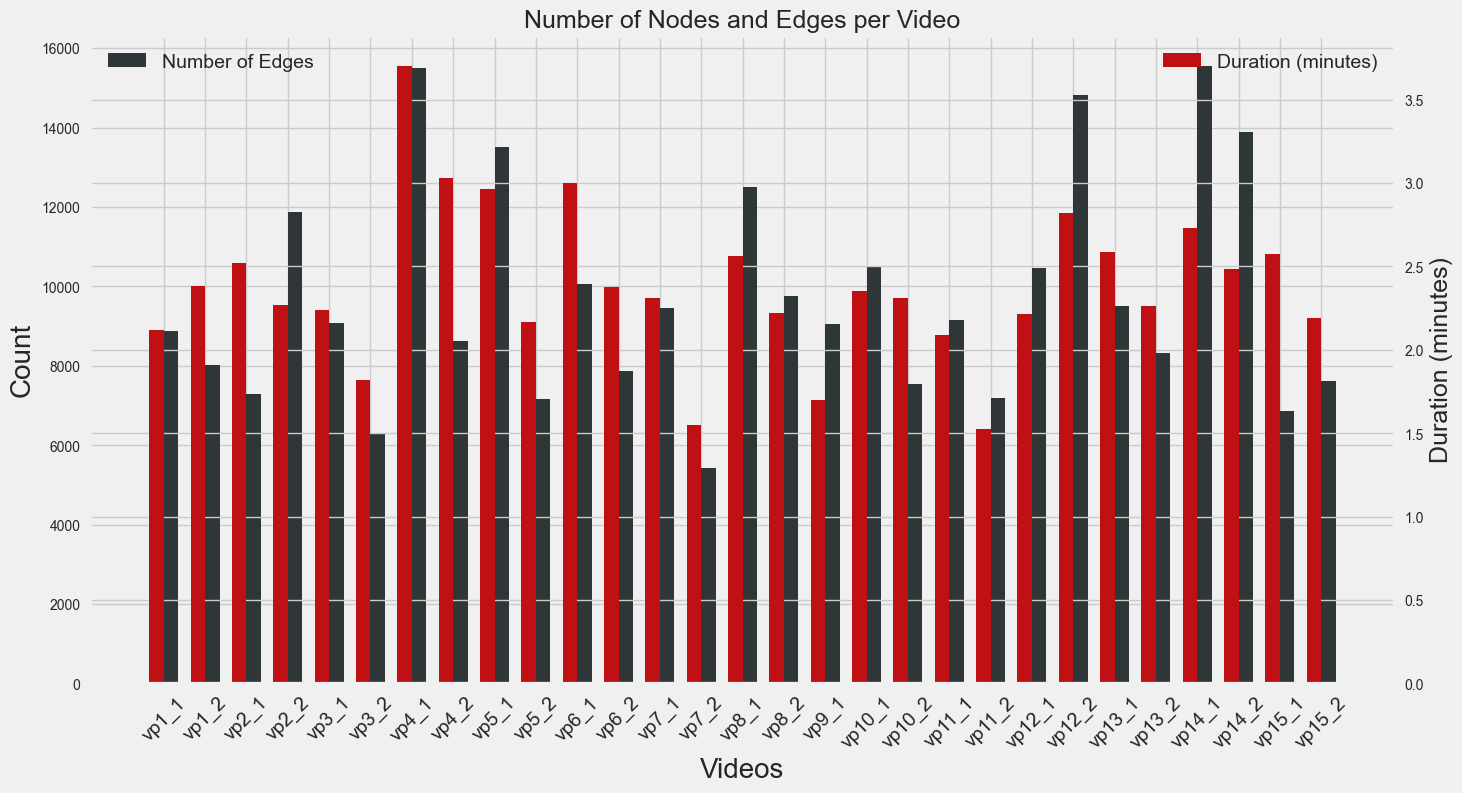
\includegraphics[width=\textwidth]{figures/05_data_statistic.png}
    \caption{Part of the statistic of the dataset}
    \label{fig:dataset_statistic}
\end{figure}

As for measurement, In our study, we utilize the \textbf{AU-ROC} and \textbf{AP} metric to evaluate and compare the performance of different models, as it provides a robust measure of a model's ability to distinguish between classes, particularly in imbalanced datasets. 

\textbf{AU-ROC (Area Under the Receiver Operating Characteristic Curve)} measures a model's classification ability by plotting the trade-off between the True Positive Rate (TPR) and False Positive Rate (FPR) across thresholds. It is calculated as: 

\[
\text{TPR} = \frac{\text{TP}}{\text{TP} + \text{FN}}, \quad \text{FPR} = \frac{\text{FP}}{\text{FP} + \text{TN}}
\]

An AU-ROC score of 1 indicates perfect classification, 0.5 implies random guessing, and values below 0.5 suggest poor performance. 
It is particularly effective for imbalanced datasets.

\textbf{Average Precision (AP)} measures a model's ability to balance precision and recall, summarizing the area under the Precision-Recall (PR) curve, here:
\begin{itemize}
    \item Precision = $\frac{\text{TP}}{\text{TP} + \text{FP}}$
    \item Recall = $\frac{\text{TP}}{\text{TP} + \text{FN}}$
\end{itemize}
It is particularly useful for imbalanced datasets, capturing the ranking quality of positive instances over negatives. AP is calculated as:

\[
\text{AP} = \sum_{i=1}^n \left( R_i - R_{i-1} \right) P_i
\]


where $P_i$ is precision and $R_i$ is recall at the $i^{th}$ threshold. An AP of 1.0 indicates perfect ranking, while 0.0 reflects completely incorrect predictions. It is widely used in tasks like object detection and retrieval.



\section{Model Performance Analysis}


The first step in the evaluation is a comparison of all models to identify the best-performing one in the basic task, which is to make a simple prediction on edge. Such task is achieved by training all the models with the video \textbf{vp01run1} and evaluating their performance using the AU-ROC metric. The whole training porcess is based on \textbf{DGB}\cite{poursafaei2022towards} The models considered in this comparison include \textbf{JODIE}, \textbf{TGN}, \textbf{DyRep}, and \textbf{CAW-N}.

The results are presented in Figure~\ref{fig:comparison} . Notably, the \textbf{CAW-N} model operates based on a random walking process, which limits its predictions to the existing graph. As a result, it does not produce separate outcomes for old and new node predictions.

As expected, the \textbf{JODIE} model demonstrates superior performance compared to the other three models, with \textbf{TGN} also delivering strong results. This aligns with the conclusions drawn in the previous chapter, reinforcing the robustness of these models.

Figure~\ref{fig:loss_comparison} provides clear evidence supporting our conclusions. The \textbf{JODIE} model demonstrates consistently strong performance with an optimal loss curve, indicating effective learning. The \textbf{TGN} model also performs well, though its final loss value is slightly higher than that of \textbf{JODIE}. In contrast, the \textbf{CAW-N} model exhibits signs of overfitting, as evidenced by its abrupt convergence to suboptimal solutions within very few epochs. Meanwhile, the \textbf{DyRep} model maintains a consistently high loss value throughout the training process, suggesting an inability to capture the underlying patterns in the dataset—indicative of underfitting.

\begin{figure}[h]
    \centering
    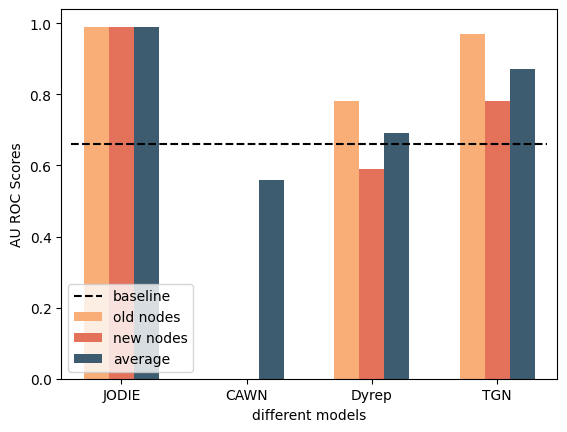
\includegraphics[width=0.6\textwidth]{figures/05_different_model_selection.png}
    \caption{The comparison between different models}
    \label{fig:comparison}
\end{figure}

\begin{figure}
    \centering
    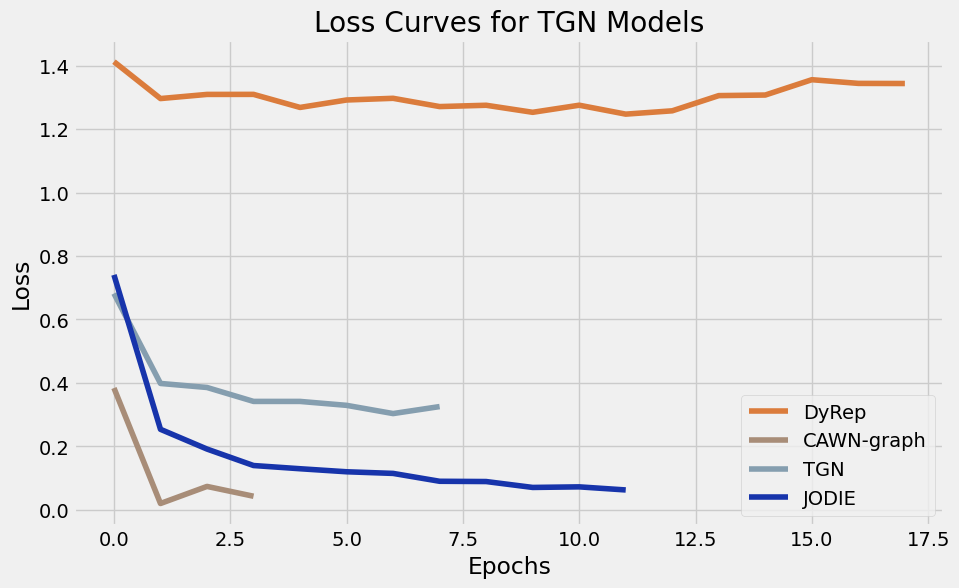
\includegraphics[width=0.8\textwidth]{figures/05_model_loss.png}
    \caption{training process between different models}
    \label{fig:loss_comparison}
\end{figure}
% the statistic of the dataset(timelenth)

\section{JODIE Results}


The decision to train the model with the original \textbf{JODIE} model serves two primary purposes. First, it allows us to validate our earlier hypothesis that JODIE exhibits superior performance across most videos in our dataset. Second, it provides a benchmark for comparison with the modified model incorporating state embeddings.

The evaluation of JODIE on individual videos demonstrates its robustness in predicting dynamic behavior, with results shown in Figure~\ref{fig:JODIE_results}. The model achieves consistent performance, with AU-ROC scores and APC approaching 1 across all original videos. This high accuracy can be attributed to the model's simplicity when edge states are excluded, relying only on single interactions per time period. Moreover, JODIE performs well in predicting both old and new nodes, indicating its ability to generalize across different node types.

However, challenges arise when training on the combined graph, which merges all videos. The increased complexity of this dataset—characterized by 15 participants, a significantly larger number of edges, and an extended duration—appears to hinder the model's performance. Despite this, JODIE remains the most effective model in our experiments when trained on graphs generated from individual videos in the dataset, further supporting its selection as a baseline.



\begin{figure}
    \centering
    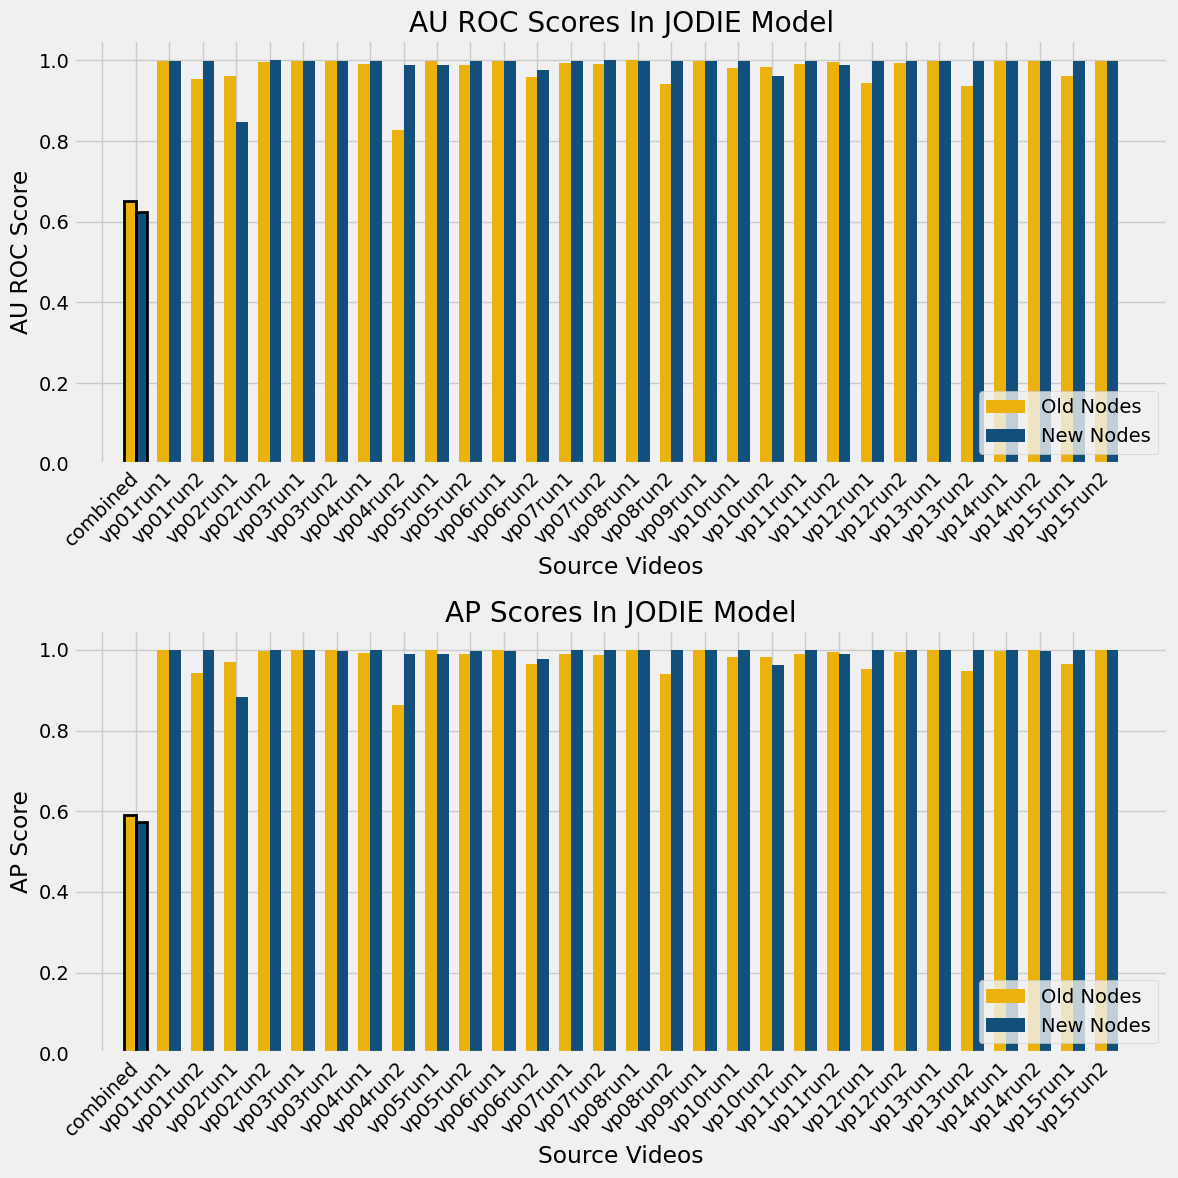
\includegraphics[width=\textwidth]{figures/05_JODIE.png}
    \caption{Dynamic Behavior Prediction Using JODIE}
    \label{fig:JODIE_results}
\end{figure}

\clearpage

\section{HMM Evaluation}



At this stage, the basic prediction tasks can already be performed on the dynamic graphs prepared for learning. However, none of the given models can predict both the edges and their corresponding states on the dynamic graphs effectively. To address this limitation, we first consider some classic models that offer the possiblity of future behavior prediction in some time-consequent datasets.

As is discussed before, we decide to evaluate the performance of Hidden Markov Models (HMM) on the same dataset. The HMM model is trained using the same dynamic graph structure as the JODIE model, with identical training and testing splits. The results are presented in Figure~\ref{fig:HMM_results}. Due to the inherent variability in the output of HMM, multiple training runs were conducted to provide a comprehensive understanding of its performance.

From the figure, it is evident that while HMM can learn from all the graphs and generate predictions for future behaviors, the results lack consistent patterns. In some cases, such as the training on \textit{vp03run1}, \textit{vp08run2}, \textit{vp10run2}, \textit{vp13run1}, and \textit{vp13run2}, peaks in the AU-ROC score are observed. However, these peaks are not replicable across different training runs on the same graphs, indicating that the HMM model lacks stability for dynamic graph prediction tasks. A similar inconsistency is also observed in the AP scores.

Although HMM offers a minimalist approach to the problem and demonstrates potential for application in dynamic graph prediction tasks, its inherent instability makes it unsuitable for real-world scenarios. The subsequent section presents our solution to this limitation by integrating state embeddings into the JODIE model.


\begin{figure}[h]
    \centering
    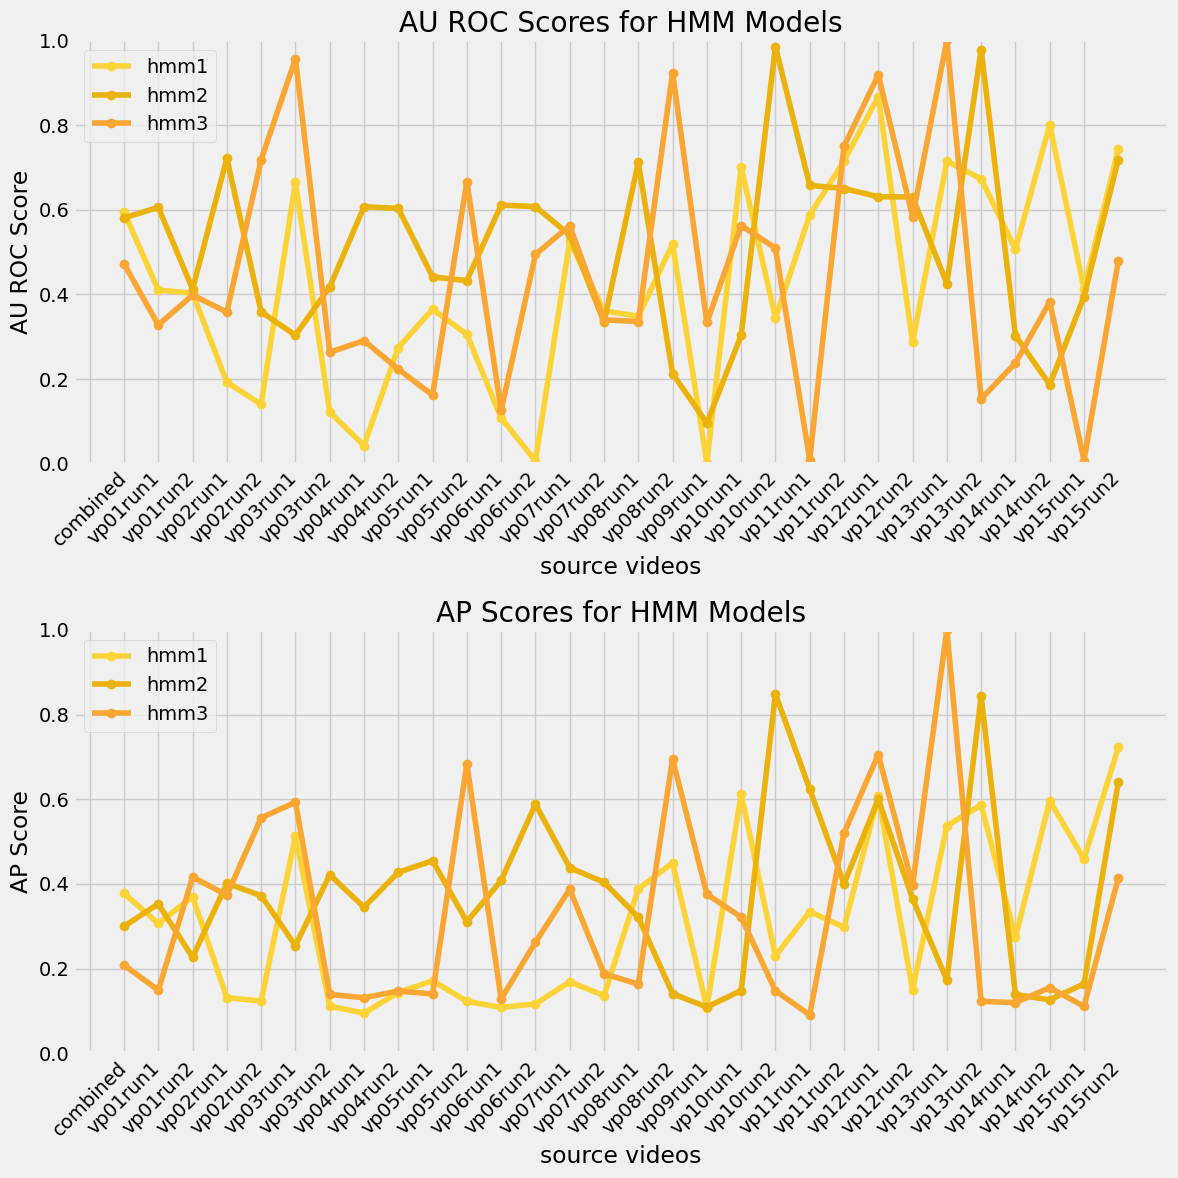
\includegraphics[width=\textwidth]{figures/05_baseline.png}
    \caption{Baseline Evaluation with Hidden Markov Models (HMM)}
    \label{fig:HMM_results}
\end{figure}


\clearpage
\section{Impact of State Embeddings}
Finally, we evaluate our proposed approach: JODIE with integrated state embeddings. The results, presented in Figure~\ref{fig:JODIE_state_embedding_results}, are derived from training the model on the same dataset as the original JODIE model, with the sole modification being the inclusion of state embeddings.

The inclusion of state embeddings in the model unsurprisingly results in a drop in AUROC and AP scores. This can be attributed to the increased complexity of the model and the introduction of additional features. However, the model continues to perform well in dynamic graph prediction, as no significant failures are observed across prediction tasks. Interestingly, the combined graph, which aggregates data from multiple participants, achieves a higher AUROC score than several single-participant graphs. This provides strong evidence that the model is capable of generalizing predictions to larger datasets. Looking ahead, this suggests that incorporating more diverse models or larger datasets could further enhance its robustness. At the same time, it hints at possible underfitting in certain training runs, where the available dataset may not be sufficient for the model’s sophisticated structure. The fact that the overall AP score is lower than the AUROC score may also support this argument. This discrepancy can be attributed to the nature of the two metrics. While AUROC focuses on the model's ability to distinguish between classes, AP emphasizes the ranking quality of positive instances over negatives. In the context of our study, the lower AP score suggests that the model pooly ranks the true positives or generates many false positives, which may be due to the complexity of the dataset and the model's inability to capture the underlying patterns.Encouragingly, the both facts highlight the model’s latent computational potential, which remains to be fully realized in the future study.

Another notable observation is the model’s superior performance in predicting new nodes compared to old ones. This aligns with the conclusion that state embeddings enhance the model’s sequential prediction capabilities. For our primary task of identifying potential driving risks, accurate prediction of new nodes is especially critical, as unexpected or previously unseen items often pose a greater hazard. Given that drivers tend to repeat their actions, the ability to reliably detect new nodes underscores the model’s importance and effectiveness in addressing safety-critical scenarios.

\begin{figure}[h]
    \centering
    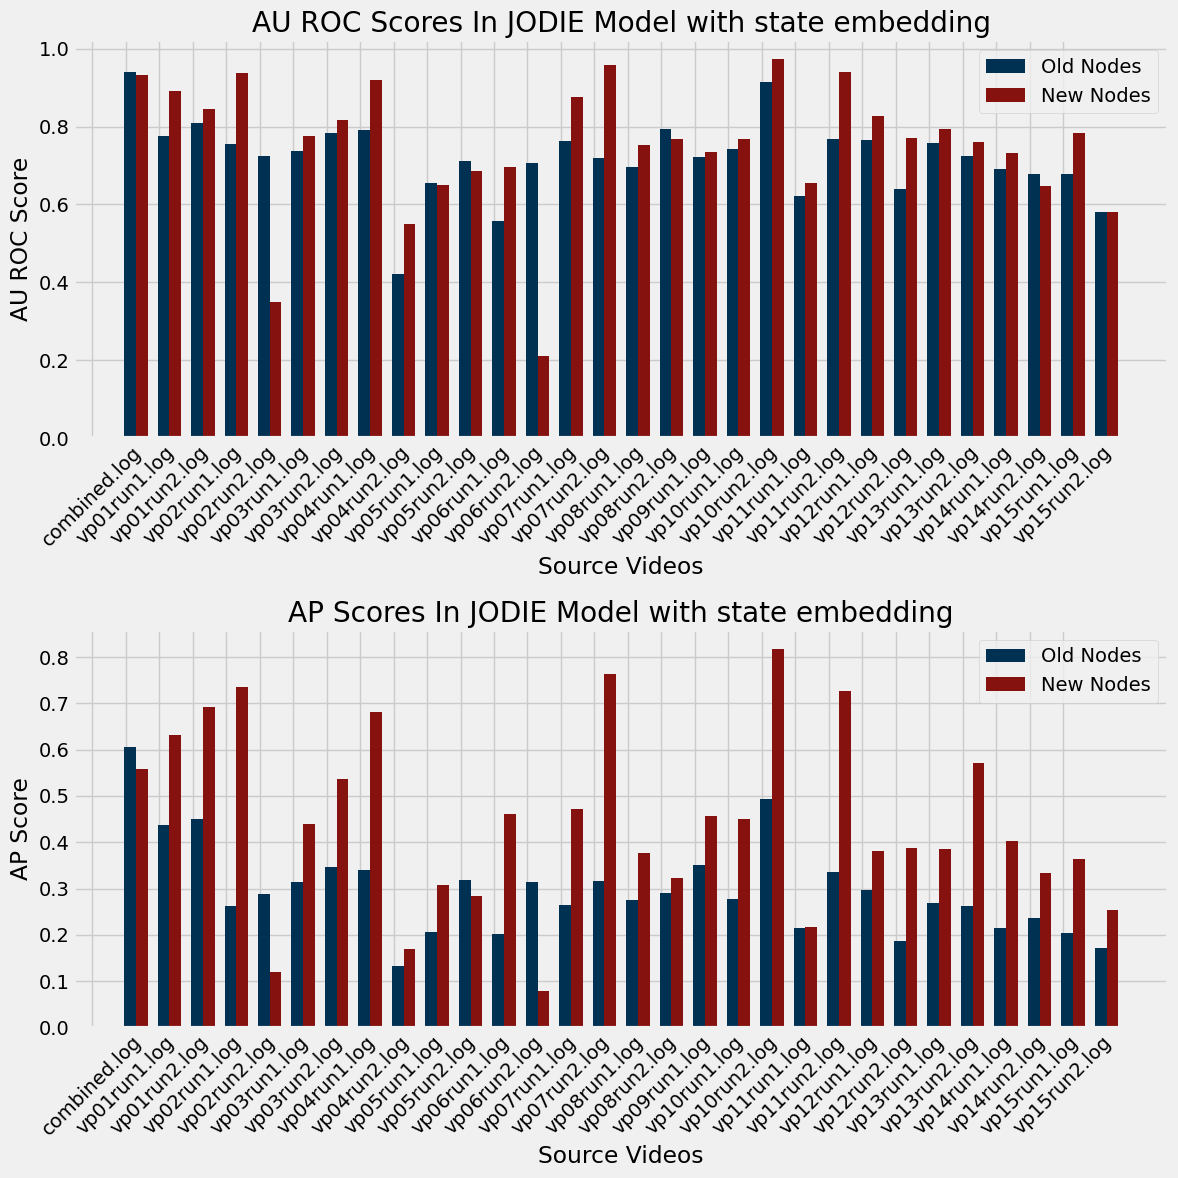
\includegraphics[width=\textwidth]{figures/05_JODIE_with_state.png}
    \caption{summery of JODIE with State Embedding}
    \label{fig:JODIE_state_embedding_results}
\end{figure}

\clearpage
% TODO:yet still our work is much better than HMM

For the comparison between our model and the HMM model, the results are shown in Figure~\ref{fig:JODIE_state_HMM_AUROC} and Figure~\ref{fig:JODIE_state_HMM_AP}. A random result pair from the previous HMM training is selected for reference. The JODIE model with state embeddings consistently outperforms the HMM model across all videos in terms of AUROC scores. Regarding AP scores, while the HMM model occasionally surpasses our approach in certain cases, our model demonstrates superior performance in many situations. This highlights the greater stability of our model compared to traditional methods, as the variance in results is significantly lower than that of HMM. Furthermore, the findings emphasize the limitations of traditional models like HMM in managing complex, dynamic datasets, reinforcing the necessity of advanced techniques such as JODIE with state embeddings.

Additional evidence supporting the stability of our model across different runs can be found in the Appendix\ref{chapter:appendixB}. These results demonstrate that our model is not generating predictions at random but instead identifies and summarizes consistent patterns and features from the dataset. This consistency further underscores the robustness of our approach and its ability to generalize effectively.

\clearpage

\begin{figure}
    \centering
    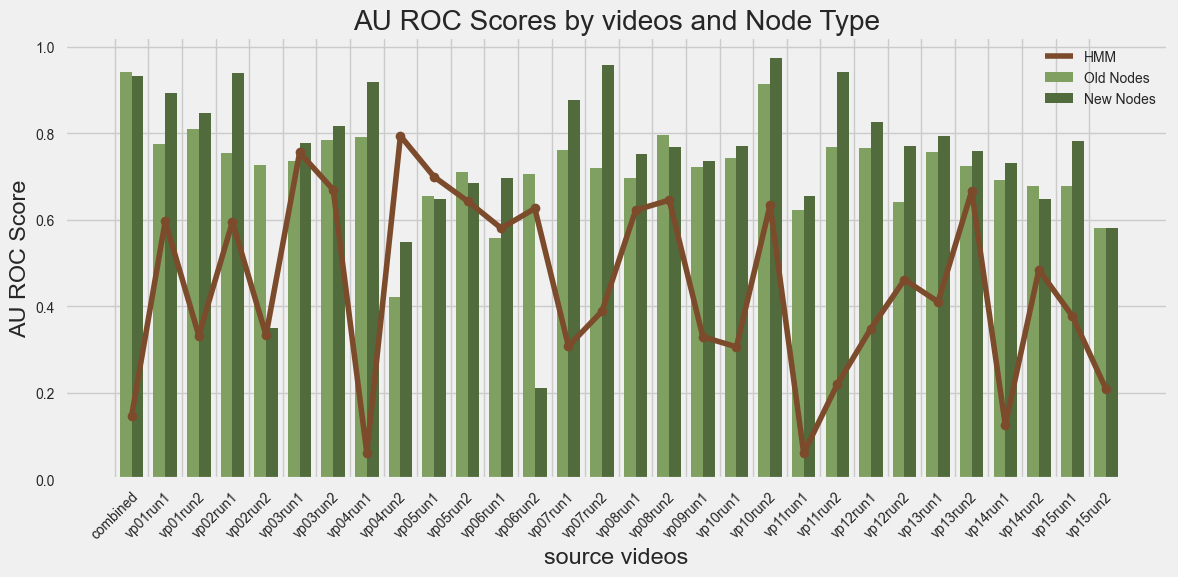
\includegraphics[width=\textwidth]{figures/05_JODIE_state_HMM_AUROC.png}
    \caption{summery of JODIE with State Embedding}
    \label{fig:JODIE_state_HMM_AUROC}
\end{figure}



\begin{figure}
    \centering
    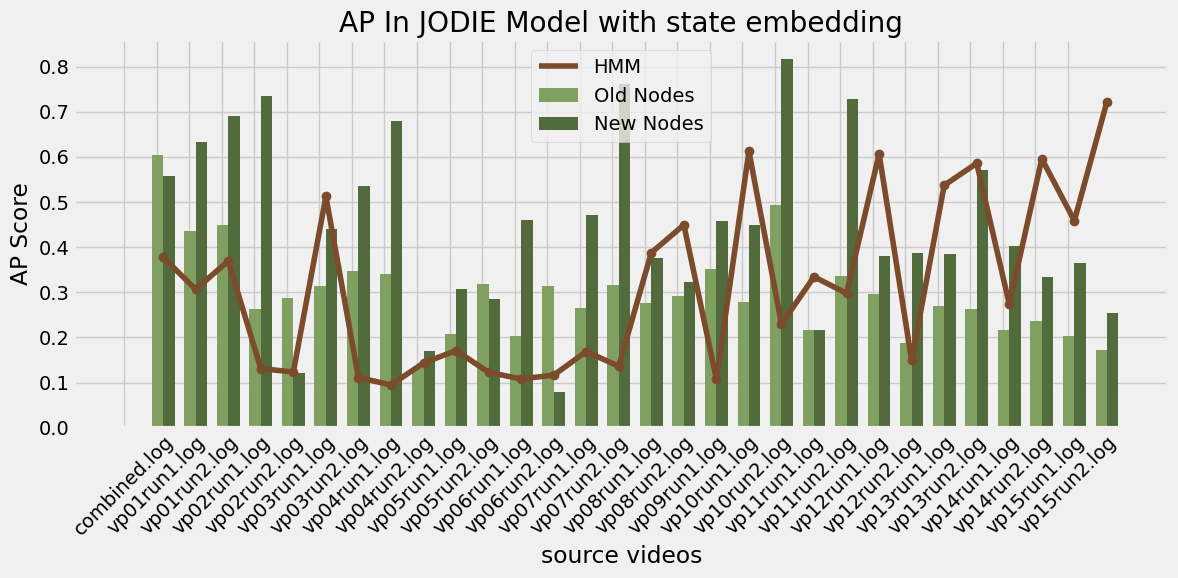
\includegraphics[width=\textwidth]{figures/05_JODIE_state_HMM_AP.png}
    \caption{summery of JODIE with State Embedding}
    \label{fig:JODIE_state_HMM_AP}
\end{figure}


\chapter{Future Work}\label{chapter:futurework}
\chapter{Conclusion}\label{chapter:conclusion}



\appendix{}

% TODO: appendix chapter
\chapter{Hidden Markov Model}\label{chapter:appendix}

If there are several additions you want to add, but they do not fit into the thesis itself, they belong here.

\section{Drive \& act dataset}

Even sections are possible, but usually only used for several elements in, e.g.\ tables, images, etc.

\chapter{Figures}
\section{Example 1}
\cmark
\section{Example 2}
\xmark

\microtypesetup{protrusion=false}
\listoffigures{}
\listoftables{}
\microtypesetup{protrusion=true}

\printglossaries
\printbibliography{}

\end{document}
